%!TEX program = xelatex
%%%%%%%%%%%%%%%%%%%%%%%这是导言部分的开始%%%%%%%%

%========= 导言部分声明文档的类型=================
\documentclass{article}

%=========导言部分可可以加载宏包=================
\usepackage{amsmath}                % 数学公式排版宏包
\usepackage{amssymb}                % 数学符号命令宏包
\usepackage{amsthm}                 % 数学定理宏包
\usepackage[UTF8]{ctex}             % 中文输入宏包
\usepackage[a4paper]{geometry}      % 页面设置宏包
\usepackage{setspace}               % 行间距宏包
\usepackage{graphicx}               % 图片宏包
\usepackage{listings}               % 代码宏包
\usepackage{xcolor}

%=========页面设置==============================
\geometry{left=2cm,right=2cm,top=2cm,bottom=2cm}
\onehalfspacing

%=========代码格式设置============================
\lstset{
    basicstyle=\tt,
    %行号
    numbers=left,
    rulesepcolor=\color{red!20!green!20!blue!20},
    escapeinside=``,
    xleftmargin=2em,xrightmargin=2em, aboveskip=1em,
    %背景框
    framexleftmargin=1.5mm,
    frame=shadowbox,
    %背景色
    backgroundcolor=\color[RGB]{245,245,244},
    %样式
    keywordstyle=\color{blue}\bfseries,
    identifierstyle=\bf,
    numberstyle=\color[RGB]{0,192,192},
    commentstyle=\it\color[RGB]{96,96,96},
    stringstyle=\rmfamily\slshape\color[RGB]{128,0,0},
    %显示空格
    showstringspaces=false
}

%=========导言部分可以定义标题信息===============
\title{组会报告}
\author{徐益}
\date{2018/4/19}

%%%%%%%%%%%%%%%%%%%%%%%这是导言部分的结束%%%%%%%%%

%%%%%%%%%%%%%%%%%%%%%%%这是正文部分的开始%%%%%%%%%
\begin{document}
	
%=========生成标题================================
\maketitle

%=========开始正文的输入==========================

%===========第一节=================
\section{本周学习内容}

1. 阅读数据处理说明文档(服务器),学习srsLTE开源库

2. 配置Linux运行环境

3. 3GPP TS 38.212

%===========第一节=================
\section{数据处理说明文档(服务器)}

\subsection{服务器数据处理流程图}
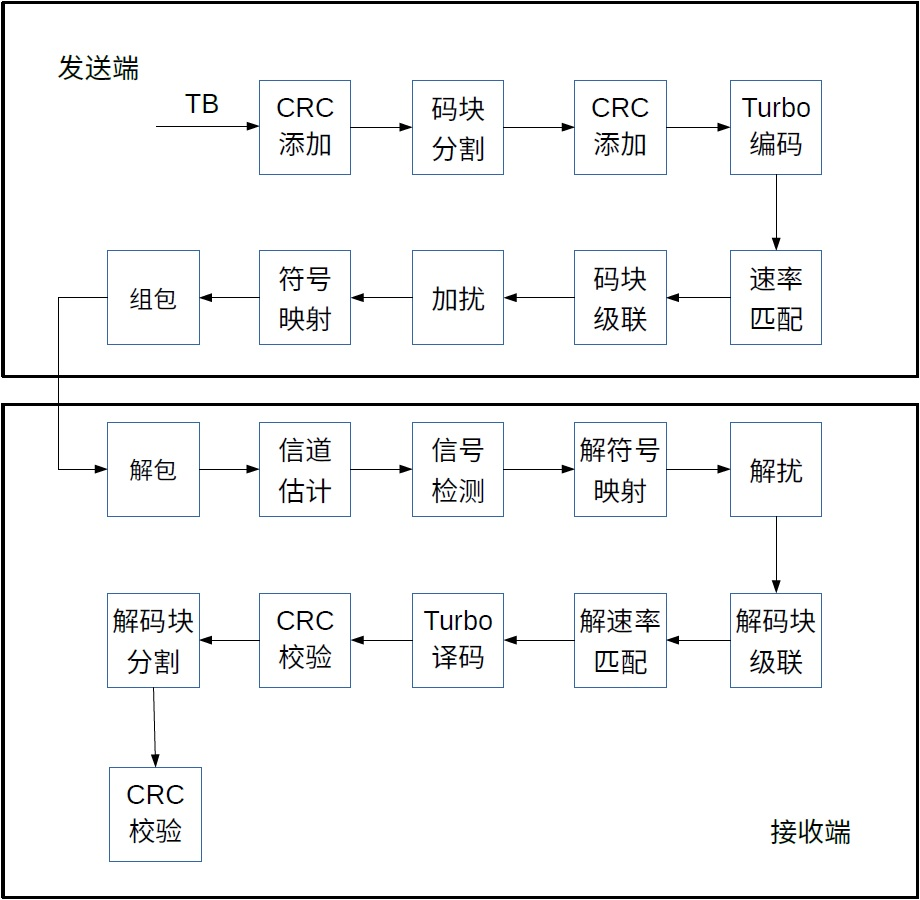
\includegraphics[width = .9\textwidth]{flowchartDataProcess.jpg}

\subsection{srsLTE开源库目录结构}
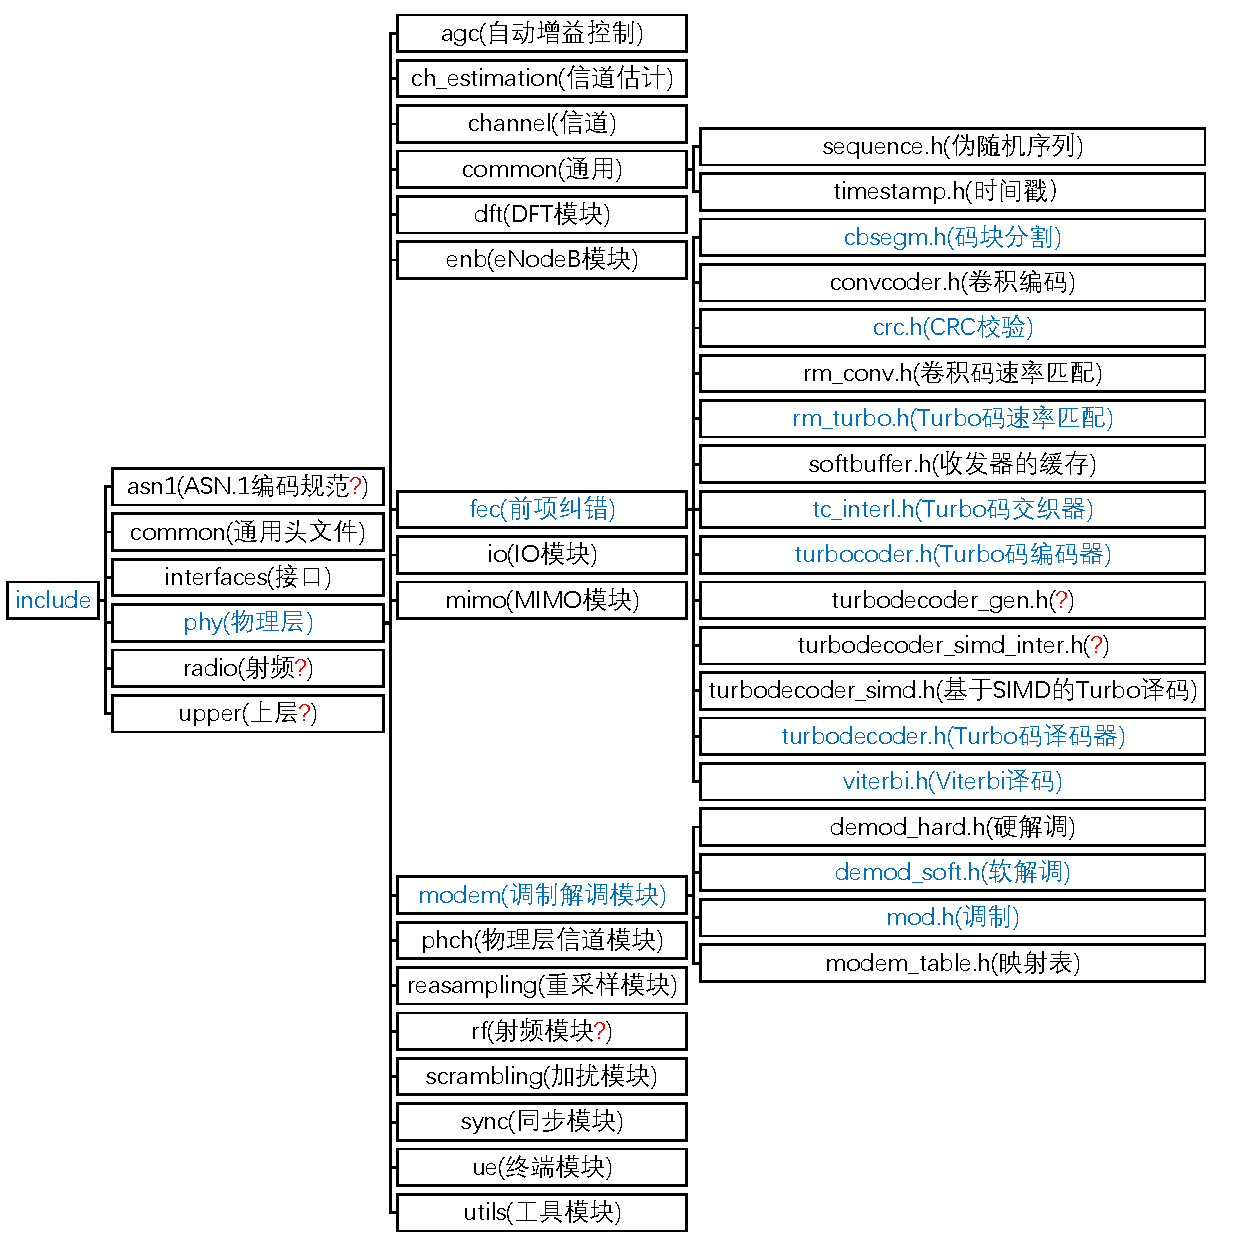
\includegraphics[width = \textwidth]{dirStructure.pdf}

%===========第二节=================
\section{配置Linux开发环境}

\subsection{Intel MKL在Linux中的安装}
1. 下载 https://software.intel.com/en-us/mkl

2. 运行 install.sh,按默认路径安装

3. 在~/.bashrc末尾添加
\lstset{language=C}
\begin{lstlisting}
source /opt/intel/bin/compilervars.sh intel64
source /opt/intel/compilers_and_libraries_2018.2.199/linux/bin/
    compilervars.sh intel64
\end{lstlisting}

\subsection{运行结果}
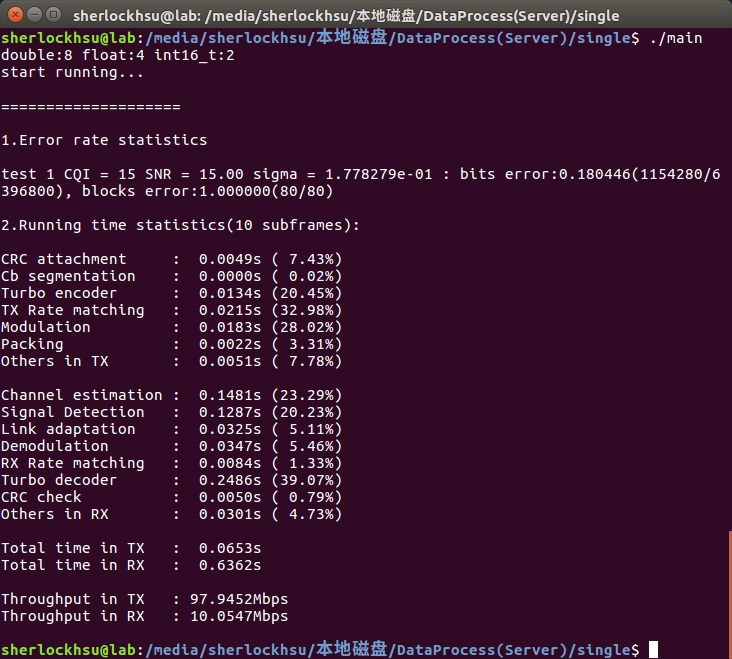
\includegraphics[width = .9\textwidth]{resSingle.jpg}

%===========第三节=================
\section{3GPP TS 38.212}

\subsection{控制信息的编码策略}
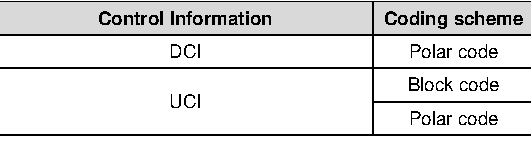
\includegraphics[width = .8\textwidth]{table_CI.pdf}

\subsection{发送端DCI信号处理流程}
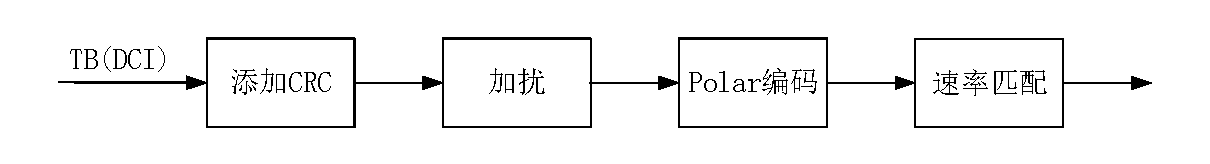
\includegraphics[width = \textwidth]{Tx_DCI_flow.pdf}

\subsection{发送端UCI信号处理流程}
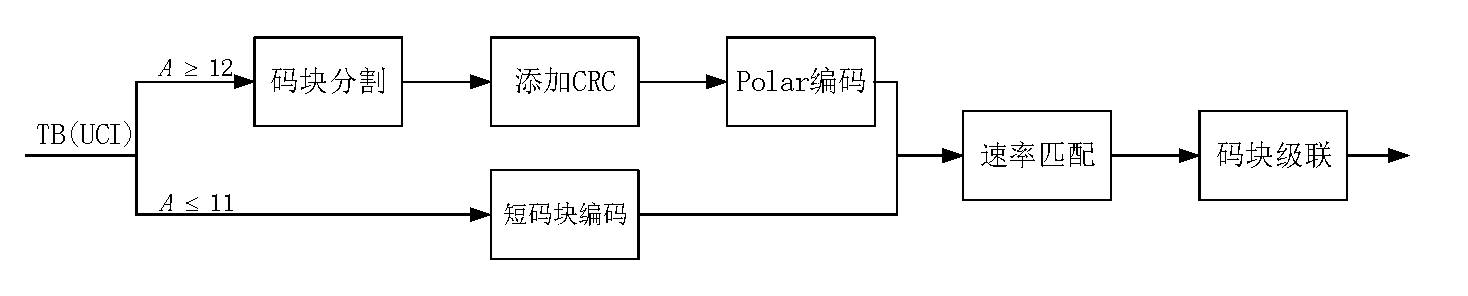
\includegraphics[width = \textwidth]{Tx_UCI_flow.pdf}

%===========存在问题=================
\section{存在问题}
1. 实现的具体部分:所有信道还是部分信道?

2. 加扰的位置?RNTI?

%===========下周计划=================
\section{下周计划}
1. 继续阅读3GPP TS 38.212

2. 尝试编写码块分割模块

\end{document}
%%%%%%%%%%%%%%%%%%%%%%%这是正文部分的结束%%%%%%%%%%%%